\documentclass[uplatex, dvipdfmx, unicode]{beamer}
\usetheme{CambridgeUS}
\usepackage{amsmath, amssymb}
\usepackage{fontawesome}
\usepackage{tikz}
\usetikzlibrary{calc}

\title{入出力の話}
\author{\texttt{@leno3s}}
\date{\today}
\institute{\url{leno3s.net}}

\begin{document}
\maketitle

\begin{frame}{もくじ}
  \tableofcontents
\end{frame}

\begin{frame}{今日の目標}
  \begin{itemize}
    \item{標準入出力を理解する.}
    \item{リダイレクトを用いたファイルの入出力ができる.(重要)}
    \item{シェル芸への思想を理解する.(発展)}
  \end{itemize}
  

\end{frame}

\begin{frame}{対象}
  \begin{itemize}
    \item{簡単なCLIでの操作(ls, cd, cat, echo, ...)はわかる}
    \item{競技プログラミングの簡単な問題が解ける}
  \end{itemize}

\end{frame}

\section{CLI使ってますか?}
\begin{frame}
  \centering
  \Huge{CLI使ってますか?}
\end{frame}

\begin{frame}
  \centering
  \Huge{使ってる人\faHandPaperO}
\end{frame}

\begin{frame}
  \centering
  \Huge{使ってない人\faHandPaperO}
\end{frame}

\begin{frame}
  \centering
  \Huge{わからない人\faHandPaperO}
\end{frame}

\begin{frame}
  \centering
  \Huge{はい}
\end{frame}

\begin{frame}
  というわけでCLIの話をします.
\end{frame}

\begin{frame}
  そもそもCLIとは?
  \begin{itemize}
    \item{Command Line Interface}
    \item{グラフィカルでない, 文字入力によるインターフェース}
  \end{itemize}
\end{frame}

\begin{frame}
  \centering
  \Huge{↓これとか,} \\
  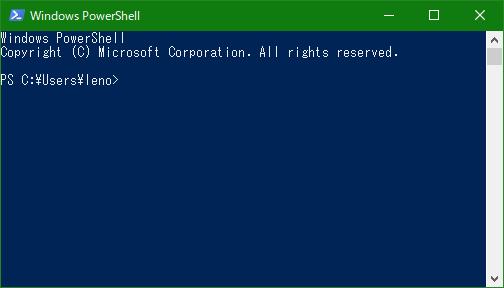
\includegraphics[keepaspectratio, scale=.5]{./img/ps.png}
\end{frame}

\begin{frame}
  \centering
  \Huge{↓これとか.} \\
  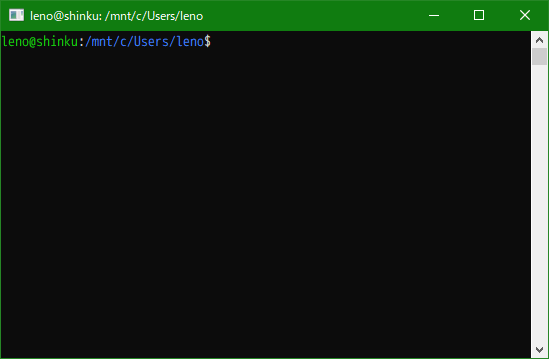
\includegraphics[keepaspectratio, scale=.5]{./img/bash.png}
\end{frame}

\begin{frame}
  普段からこんな感じで使っていると思います.
  
  \centering
  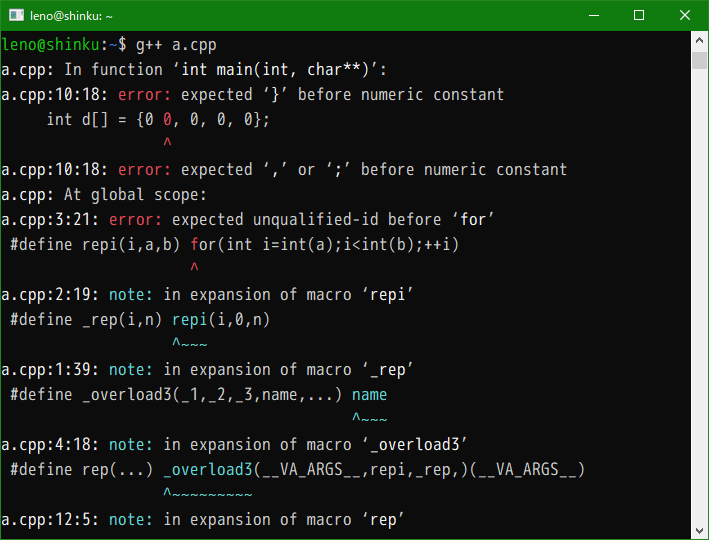
\includegraphics[keepaspectratio, scale=.5]{./img/console.png}
\end{frame}

\begin{frame}
  競プロではあるある風景ですね. (ほんまか?)
\end{frame}

\begin{frame}
  ---ところでそろそろICPC予選ですね.
\end{frame}

\begin{frame}
  ICPCでは, テストケースがテキストファイルで与えられます.\\
  (提出も, 出力結果のテキストファイルです.)
\end{frame}

\begin{frame}{}
  \centering
  \Huge{この形式のコンテストに参加した事がある人\faHandPaperO}
\end{frame}

\begin{frame}{}
  fopen()とか使うのめんどくさいよね... \\
  (普段みたいにcin/cout, scanf/printfでやりたいよね)
\end{frame}

\begin{frame}{というわけで}
  標準入出力について, お話します.
\end{frame}

\section{標準入出力って?}
\begin{frame}
  \centering
  \Huge{標準入出力についてご存知の人\faHandPaperO}
\end{frame}

\begin{frame}
  \begin{quote}
    標準ストリーム(英: standard streams)とは、UNIXやUnix系オペレーティングシステム (OS) において、プログラムの活動実体であるプロセスとその実行環境(通常は端末)の間の接続として、(プロセスから見ると)あらかじめ確立されている入出力チャネル(パイプ (コンピュータ))である。OSのカーネルではなくシェルで実装されている機能だが、広く使われているため標準化されている。UNIXやUnix系OSでは3つの入出力があり、標準入力(英: standard input)、標準出力(英: standard output)、標準エラー出力(英: standard error)である。
  \end{quote}
  \small{標準ストリーム - Wikipedia\footnote{https://ja.wikipedia.org/wiki/標準ストリーム}より.}
\end{frame}

\begin{frame}
  \centering
  \Huge{('$\mathrm{\omega}$')????????}
\end{frame}

\begin{frame}
  \begin{quote}
    標準ストリームとは、UNIXやUnix系オペレーティングシステム (OS) において、
    \alert{プログラムの活動実体であるプロセスとその実行環境(通常は端末)の間の接続}として、
    (プロセスから見ると)あらかじめ確立されている\alert{入出力チャネル}(パイプ (コンピュータ))である。 \\
    OSのカーネルではなくシェルで実装されている機能だが、広く使われているため標準化されている。
    UNIXやUnix系OSでは3つの入出力があり、\alert{標準入力、標準出力、
    標準エラー出力}である。
  \end{quote}
\end{frame}

\begin{frame}{重要ポイント}
  \begin{itemize}
    \item{なんかプロセス間の通信に使ってるらしい}
    \item{標準入力, 出力, エラー出力がある}
    \item{\alert{ST}andar\alert{D} \alert{IN}put, \alert{ST}andar\alert{D} \alert{OUT},
      \alert{ST}andar\alert{D} \alert{ERR}or}
  \end{itemize}
\end{frame}

\section{/dev/ptsの話}

\begin{frame}
  \Huge{\alert{/dev/pts/の話}}
\end{frame}

\begin{frame}
  \Large{\alert{ここからLinux/Unix基準の話をします}\faLinux} \\
  \vspace{0.2in}

  \normalsize
  環境の無い人は WSL や MSYS2 でも大丈夫, Cygwinは確認してない \\
  コマンド交えつつ話すので, 手元で実行してね
\end{frame}

\begin{frame}{/dev/って?}
  /以下のディレクトリの1つ \\
  \vspace{0.2in}
  ここにls /devの画像
\end{frame}

\begin{frame}{/dev/って?}
  \begin{itemize}
    \item{\alert{dev}iceのdev}
    \item{装置の意味}
    \item{Linux/Unixで, デバイスのための疑似ファイルが置かれる}
  \end{itemize}
\end{frame}

\begin{frame}{疑似ファイルの例}
  \begin{itemize}
    \item{/dev/stdin}
    \item{/dev/stdout}
    \item{/dev/stderr}
    \item{/dev/null}
    \item{/dev/zero}
    \item{/dev/(u)random}
  \end{itemize}
  \vspace{0.2in}
  など\ 実際はもっといっぱいある\footnote{\$ ls /dev/ して見れる 見てね}
\end{frame}

\begin{frame}{/dev/stdinを追ってみる}
  \$ ls -l /dev/stdin でstdinの情報が見れる \\
  \vspace{0.2in}
  {
    \centering
    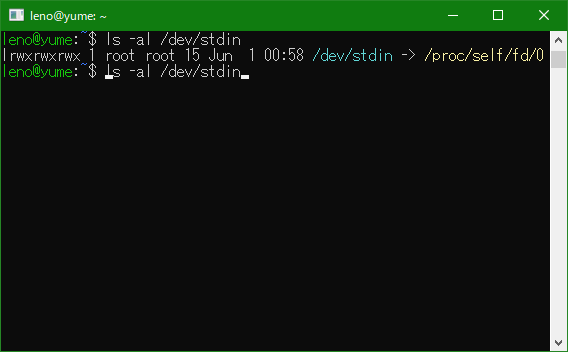
\includegraphics[keepaspectratio, scale=.5]{./img/stdin.png} \\
  }
  どうやら/proc/self/fd/0へのリンクらしい \\
\end{frame}

\begin{frame}{/dev/stdinを追ってみる}
  同様に\$ ls -l /proc/self/fd/0 する \\
  \vspace{0.2in}
  {
    \centering
    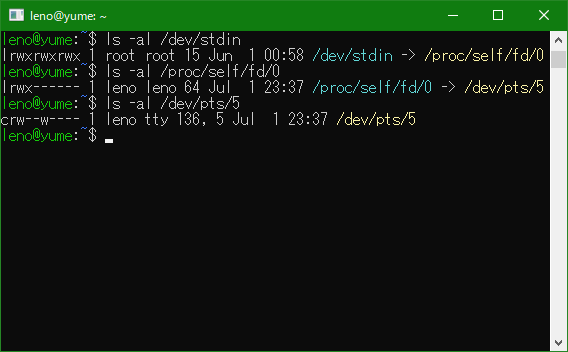
\includegraphics[keepaspectratio, scale=.5]{./img/self.png} \\
  }
  /dev/pts/1 へのリンクらしい (ここは環境によって変わります)
\end{frame}

\begin{frame}
  同様に\$ ls -l /dev/pts/1 する \\
  \vspace{0.2in}
  {
    \centering
    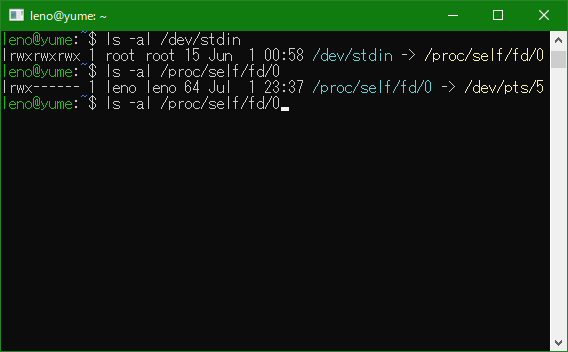
\includegraphics[keepaspectratio, scale=.5]{./img/pts.png} \\
  }
  これが本体, 数字部は...後で説明します.
\end{frame}

\begin{frame}{ttyコマンド}
  実はこの番号を調べるコマンドがある \\
  \vspace{0.2in}
  \$ tty \\
  /dev/pts/1
\end{frame}

\begin{frame}{ttyコマンド}
  もう一つウィンドウを開いて\$ ttyしてみる\\
  \vspace{0.2in}
  \$ tty \\
  /dev/pts/2
\end{frame}

\begin{frame}{ttyコマンド}
  \centering
  \alert{\Huge{!!!違う番号になった!!!}}
\end{frame}

\begin{frame}{ttyコマンド}
  ポイント
  \begin{itemize}
    \item{この番号によってウィンドウを識別している}
    \item{なんかすごいぎじゅつでウィンドウごとにstdin/out/errの番号が変わる}
  \end{itemize}
\end{frame}

\subsection{補足}
\begin{frame}{補足}
  Q. ttyって何よ \\
  A. \alert{T}ele \alert{TY}pewriter
\end{frame}

\begin{frame}{補足}
  
  印刷電信機, 昔はこれで通信をしていた. $\rightarrow$ 通信端末
  {
    \centering
    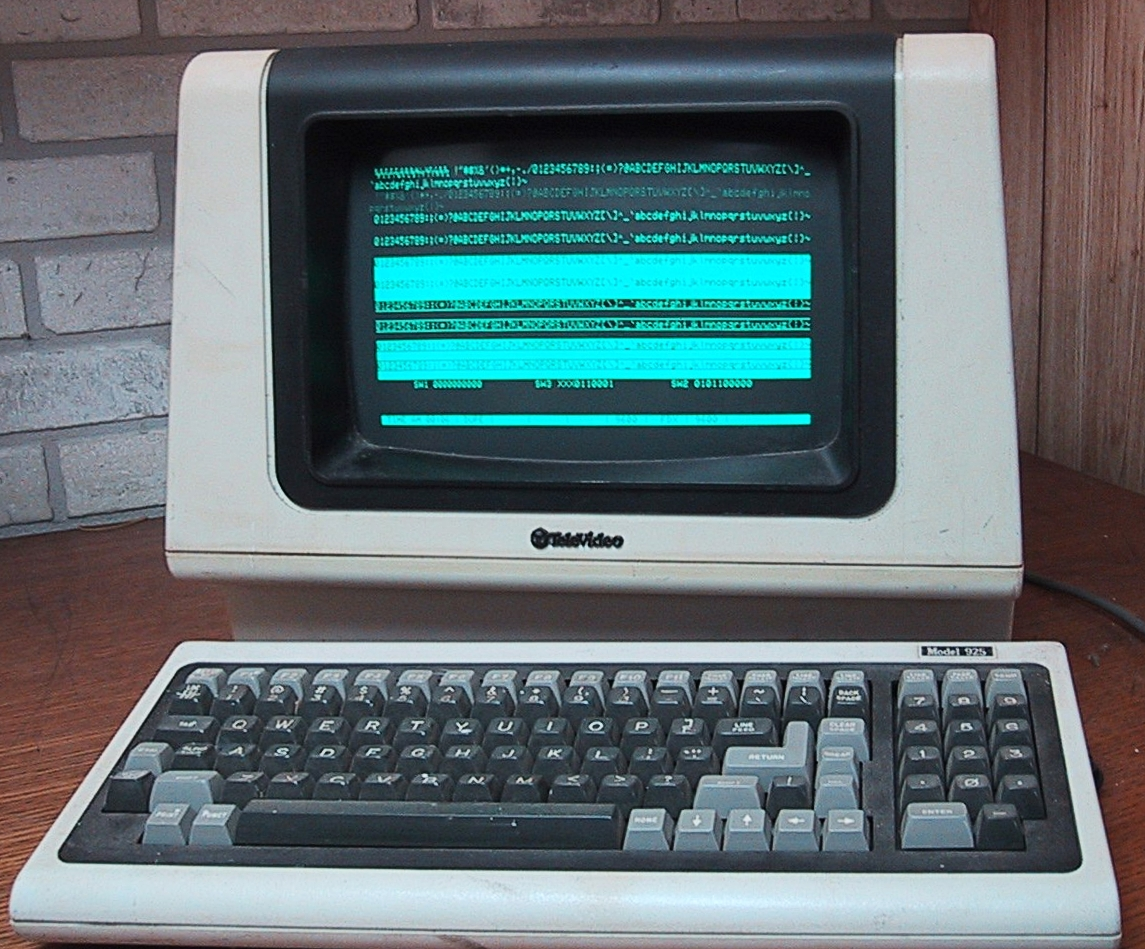
\includegraphics[keepaspectratio, scale=.18]{./img/tty.jpg} \\
  }
  \footnote*{\scriptsize 画像は\url{https://commons.wikimedia.org/wiki/File:Televideo925Terminal.jpg}}
\end{frame}

\begin{frame}{補足}
  ユーザーがコマンドを打ち込み, 結果を出力する様子がこれと似ている

  \ \ $\rightarrow$ 端末, Terminal
\end{frame}

\begin{frame}{補足}
  しかし, 今あるウィンドウは実際の端末ではない\\
  \ \ $\rightarrow$ Pseudo TTY(仮想端末) \\
  \ \ $\rightarrow$ pts
\end{frame}

\begin{frame}{補足}
  \centering
  \Huge
  $\downarrow$ 仮想端末 $\downarrow$ \\
  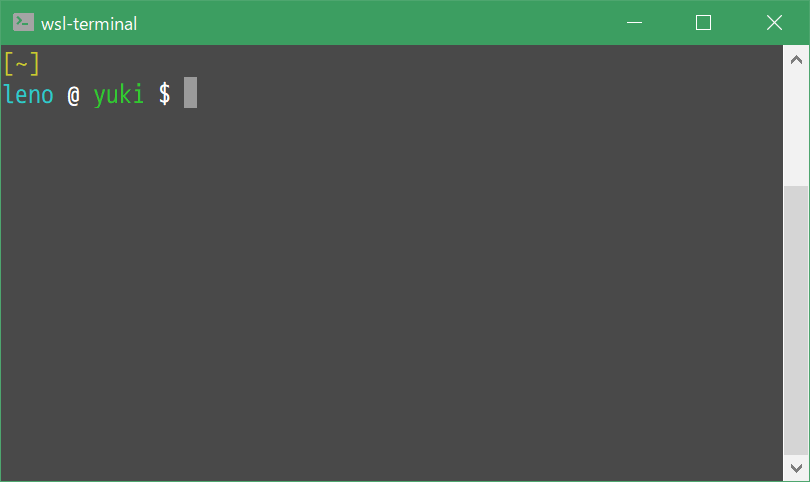
\includegraphics[keepaspectratio, scale=.5]{./img/ptty.png}
\end{frame}

\begin{frame}{補足}
  ウィンドウの表示や標準出力を表示, キーボード入力を取得したりする \\
  \alert{コマンドの解釈はしない} \\
  \ \ $\rightarrow$ これは\alert{シェル}の機能
\end{frame}

\begin{frame}{補足}
  シェル
  \begin{itemize}
    \item{bash, dash, tcsh, fish, ...}
    \item{入力されたコマンドを解釈して実行する}
    \item{カーネルを直接操作から保護する$\rightarrow$殻っぽい$\rightarrow$シェル}
  \end{itemize}
\end{frame}

\begin{frame}{補足2}
  /proc/self/fd/[0-9]のfdってなによ \\
  \ \ $\rightarrow$ File Descriptor \\
  \ \ $\rightarrow$ システムを介してファイルを扱うための鍵
\end{frame}

\begin{frame}{補足2}
  stdin/out/errに0/1/2が必ず割り当てられる \\
  他のファイルをプログラムがopen等するとfdが生成される \\
  \ \ $\rightarrow$ systemcallのopen()の返り値がこのint値
\end{frame}

\begin{frame}
  \centering
  補足終わり
\end{frame}

\subsection{}
\begin{frame}{ここで疑問}
  違う番号の/dev/pts/[0-9]*に書き込みをしたらどうなるのか?
\end{frame}

\begin{frame}{実際にやってみる}
  \begin{itemize}
    \item{vimやnano等での書き込みはできない}
    \item{\$ echo hogeしてもその端末の標準入力へ流れる}
  \end{itemize}
\end{frame}

\begin{frame}{リダイレクト}
  出力先を変えるコマンド(嘘)\footnote{これはシェルの機能であってコマンドではない}がある \\
  \$ echo hoge \alert{$>$ ./out.txt} \\
  で./out.txtへと出力することができる \\
  \vspace{.2in}
  \alert{!!!! 出力先に指定したファイルは上書きされるので注意 !!!!}
\end{frame}

\begin{frame}{リダイレクト}
  \$ echo hoge \alert{$>>$ ./out.txt} \\
  $>>$で追記になる \\
  (ファイルの末尾へ書き込む)
\end{frame}

\begin{frame}{やってみよう!}
  \$ echo hoge $>$ /dev/pts/2 \\
  (端末の番号は各自変えてね)
\end{frame}

\begin{frame}{やってみよう!}
  できましたか?どうなりましたか?\faHandPaperO
\end{frame}

\begin{frame}{やってみよう!}
  \$ command \alert{$>$ to/file/path} \\
  が標準出力先をto/file/pathへ向けている \\
  $\rightarrow$ ファイルへの保存ができる! \\
  \vspace{.5cm}
\end{frame}

\begin{frame}{図解1}
  \centering
  \$ echo hoge
  \begin{figure}[h]
    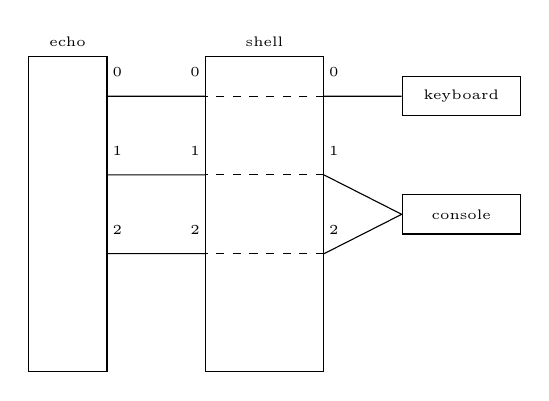
\begin{tikzpicture}[scale=.5]
      \draw (0, 0) node [draw,rectangle,minimum width=1cm,minimum height=4cm,label={\tiny echo}] (p) {}
        ($(p.east) + (0, 3)$) coordinate (pin) node [label={\tiny 0}, right](){}
        ($(p.east) + (0, 1)$) coordinate (pout) node [label={\tiny 1}, right](){}
        ($(p.east) + (0,-1)$) coordinate (perr) node [label={\tiny 2}, right](){};
      \draw (5, 0) node [draw,rectangle,minimum width=1.5cm,minimum height=4cm,label={\tiny shell}] (sh) {}
        ($(sh.east) + (0, 3)$) coordinate (srin) node [label={\tiny 0}, right](){}
        ($(sh.east) + (0, 1)$) coordinate (srout) node [label={\tiny 1}, right](){}
        ($(sh.east) + (0,-1)$) coordinate (srerr) node [label={\tiny 2}, right](){}
        ($(sh.west) + (0, 3)$) coordinate (slin) node [label={\tiny 0}, left](){}
        ($(sh.west) + (0, 1)$) coordinate (slout) node [label={\tiny 1}, left](){}
        ($(sh.west) + (0,-1)$) coordinate (slerr) node [label={\tiny 2}, left](){};
      \draw (10, 3) node [draw,rectangle,minimum width=1.5cm,minimum height=.5cm] (key) {\tiny keyboard}
        (key.west) coordinate (key);
      \draw (10, 0) node [draw,rectangle,minimum width=1.5cm,minimum height=.5cm] (con) {\tiny console}
        (con.west) coordinate (con);
      \draw
        (srin) -- (key)
        (srout) -- (con)
        (srerr) -- (con)
        (pin) -- (slin)
        (pout) -- (slout)
        (perr) -- (slerr);
      \draw[dashed]
        (srin) -- (slin)
        (srout) -- (slout)
        (srerr) -- (slerr);
    \end{tikzpicture}
  \end{figure}
  KBが標準入力に, 標準(エラー)出力がコンソールに繋がる
\end{frame}

\begin{frame}{図解2}
  \centering
  \$ echo hoge $>$ out.txt
  \begin{figure}[h]
    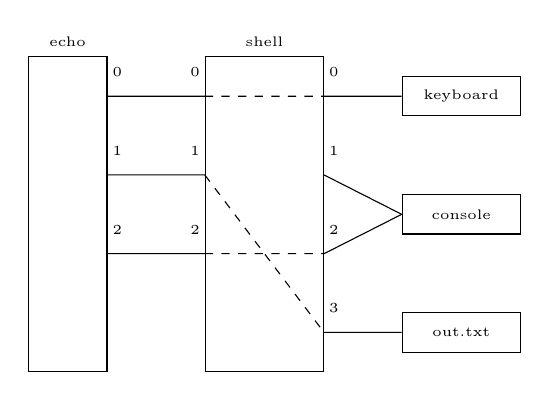
\begin{tikzpicture}[scale=.5]
      \draw (0, 0) node [draw,rectangle,minimum width=1cm,minimum height=4cm,label={\tiny echo}] (p) {}
        ($(p.east) + (0, 3)$) coordinate (pin) node [label={\tiny 0}, right](){}
        ($(p.east) + (0, 1)$) coordinate (pout) node [label={\tiny 1}, right](){}
        ($(p.east) + (0,-1)$) coordinate (perr) node [label={\tiny 2}, right](){};
      \draw (5, 0) node [draw,rectangle,minimum width=1.5cm,minimum height=4cm,label={\tiny shell}] (sh) {}
        ($(sh.east) + (0, 3)$) coordinate (srin) node [label={\tiny 0}, right](){}
        ($(sh.east) + (0, 1)$) coordinate (srout) node [label={\tiny 1}, right](){}
        ($(sh.east) + (0,-1)$) coordinate (srerr) node [label={\tiny 2}, right](){}
        ($(sh.east) + (0,-3)$) coordinate (sr3) node [label={\tiny 3}, right](){}
        ($(sh.west) + (0, 3)$) coordinate (slin) node [label={\tiny 0}, left](){}
        ($(sh.west) + (0, 1)$) coordinate (slout) node [label={\tiny 1}, left](){}
        ($(sh.west) + (0,-1)$) coordinate (slerr) node [label={\tiny 2}, left](){};
      \draw (10, 3) node [draw,rectangle,minimum width=1.5cm,minimum height=.5cm] (key) {\tiny keyboard}
        (key.west) coordinate (key);
      \draw (10, 0) node [draw,rectangle,minimum width=1.5cm,minimum height=.5cm] (con) {\tiny console}
        (con.west) coordinate (con);
      \draw (10, -3) node [draw,rectangle,minimum width=1.5cm,minimum height=.5cm] (f) {\tiny out.txt}
        (f.west) coordinate (file);
      \draw
        (srin) -- (key)
        (srout) -- (con)
        (srerr) -- (con)
        (pin) -- (slin)
        (pout) -- (slout)
        (perr) -- (slerr)
        (sr3) -- (file);
      \draw[dashed]
        (slout) -- (sr3)
        (slin) -- (srin)
        (slerr) -- (srerr);
    \end{tikzpicture}
  \end{figure}
  echo の標準出力が fd=3(out.txt) へ向かう
\end{frame}


\begin{frame}{標準入力}
  入力のリダイレクトもできる \\
  \$ grep regex $<$ hoge.txt \\
  \vspace{.2in}
  普段はキーボードから入力を待つところを, ファイルの内容を入力とすることができる. \\
  \ \ $\rightarrow$ !!! ファイルからの標準入力に使えるのでは !!! \\
\end{frame}

\begin{frame}{ちょっと補足}
  リダイレクトにはFile Descriptorを指定できる \\
  e.g.)
  \begin{itemize}
    \item{echo hoge 0$>$\&1}
    \item{curl example.com $>$ file.txt 2$>$\&1 }
  \end{itemize}
\end{frame}

\begin{frame}{図解3}
  \centering
  \$ ./a.out $<$ in.txt $>$ out.txt
  \begin{figure}[h]
    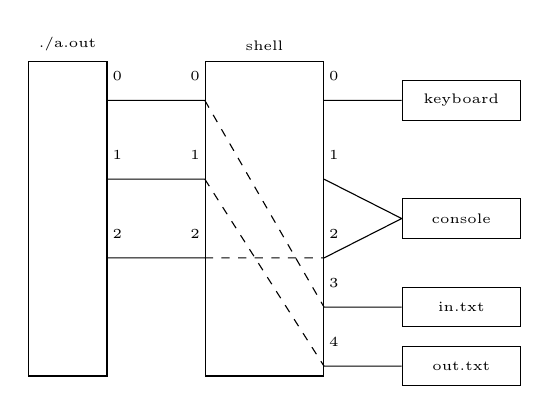
\begin{tikzpicture}[scale=.5]
      \draw (0, 0) node [draw,rectangle,minimum width=1cm,minimum height=4cm,label={\tiny ./a.out}] (p) {}
        ($(p.east) + (0, 3)$) coordinate (pin) node [label={\tiny 0}, right](){}
        ($(p.east) + (0, 1)$) coordinate (pout) node [label={\tiny 1}, right](){}
        ($(p.east) + (0,-1)$) coordinate (perr) node [label={\tiny 2}, right](){};
      \draw (5, 0) node [draw,rectangle,minimum width=1.5cm,minimum height=4cm,label={\tiny shell}] (sh) {}
        ($(sh.east) + (0, 3)$) coordinate (srin) node [label={\tiny 0}, right](){}
        ($(sh.east) + (0, 1)$) coordinate (srout) node [label={\tiny 1}, right](){}
        ($(sh.east) + (0,-1)$) coordinate (srerr) node [label={\tiny 2}, right](){}
        ($(sh.east) + (0,-2.25)$) coordinate (sr3) node [label={\tiny 3}, right](){}
        ($(sh.east) + (0,-3.75)$) coordinate (sr4) node [label={\tiny 4}, right](){}
        ($(sh.west) + (0, 3)$) coordinate (slin) node [label={\tiny 0}, left](){}
        ($(sh.west) + (0, 1)$) coordinate (slout) node [label={\tiny 1}, left](){}
        ($(sh.west) + (0,-1)$) coordinate (slerr) node [label={\tiny 2}, left](){};
      \draw (10, 3) node [draw,rectangle,minimum width=1.5cm,minimum height=.5cm] (key) {\tiny keyboard}
        (key.west) coordinate (key);
      \draw (10, 0) node [draw,rectangle,minimum width=1.5cm,minimum height=.5cm] (con) {\tiny console}
        (con.west) coordinate (con);
      \draw (10, -2.25) node [draw,rectangle,minimum width=1.5cm,minimum height=.5cm] (f) {\tiny in.txt}
        (f.west) coordinate (in);
      \draw (10, -3.75) node [draw,rectangle,minimum width=1.5cm,minimum height=.5cm] (f) {\tiny out.txt}
        (f.west) coordinate (out);
      \draw
        (srin) -- (key)
        (srout) -- (con)
        (srerr) -- (con)
        (pin) -- (slin)
        (pout) -- (slout)
        (perr) -- (slerr)
        (sr3) -- (in)
        (sr4) -- (out);
      \draw[dashed]
        (slin) -- (sr3)
        (slout) -- (sr4)
        (slerr) -- (srerr);
    \end{tikzpicture}
  \end{figure}
  echo への標準入力に in.txt が渡される
\end{frame}

\begin{frame}{図解4}
  \centering
  \$ ./a.out in.txt $>$ out.txt 2$>$\&1
  \begin{figure}[h]
    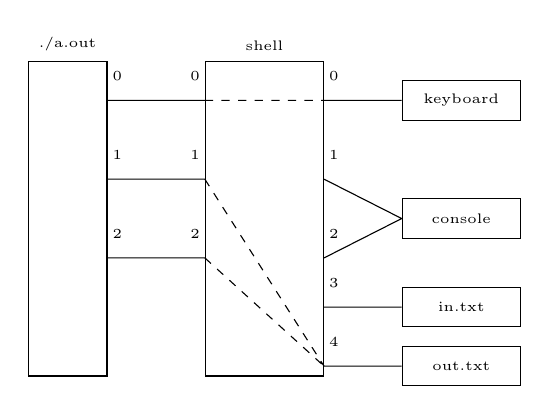
\begin{tikzpicture}[scale=.5]
      \draw (0, 0) node [draw,rectangle,minimum width=1cm,minimum height=4cm,label={\tiny ./a.out}] (p) {}
        ($(p.east) + (0, 3)$) coordinate (pin) node [label={\tiny 0}, right](){}
        ($(p.east) + (0, 1)$) coordinate (pout) node [label={\tiny 1}, right](){}
        ($(p.east) + (0,-1)$) coordinate (perr) node [label={\tiny 2}, right](){};
      \draw (5, 0) node [draw,rectangle,minimum width=1.5cm,minimum height=4cm,label={\tiny shell}] (sh) {}
        ($(sh.east) + (0, 3)$) coordinate (srin) node [label={\tiny 0}, right](){}
        ($(sh.east) + (0, 1)$) coordinate (srout) node [label={\tiny 1}, right](){}
        ($(sh.east) + (0,-1)$) coordinate (srerr) node [label={\tiny 2}, right](){}
        ($(sh.east) + (0,-2.25)$) coordinate (sr3) node [label={\tiny 3}, right](){}
        ($(sh.east) + (0,-3.75)$) coordinate (sr4) node [label={\tiny 4}, right](){}
        ($(sh.west) + (0, 3)$) coordinate (slin) node [label={\tiny 0}, left](){}
        ($(sh.west) + (0, 1)$) coordinate (slout) node [label={\tiny 1}, left](){}
        ($(sh.west) + (0,-1)$) coordinate (slerr) node [label={\tiny 2}, left](){};
      \draw (10, 3) node [draw,rectangle,minimum width=1.5cm,minimum height=.5cm] (key) {\tiny keyboard}
        (key.west) coordinate (key);
      \draw (10, 0) node [draw,rectangle,minimum width=1.5cm,minimum height=.5cm] (con) {\tiny console}
        (con.west) coordinate (con);
      \draw (10, -2.25) node [draw,rectangle,minimum width=1.5cm,minimum height=.5cm] (f) {\tiny in.txt}
        (f.west) coordinate (in);
      \draw (10, -3.75) node [draw,rectangle,minimum width=1.5cm,minimum height=.5cm] (f) {\tiny out.txt}
        (f.west) coordinate (out);
      \draw
        (srin) -- (key)
        (srout) -- (con)
        (srerr) -- (con)
        (pin) -- (slin)
        (pout) -- (slout)
        (perr) -- (slerr)
        (sr3) -- (in)
        (sr4) -- (out);
      \draw[dashed]
        (slin) -- (srin)
        (slout) -- (sr4)
        (slerr) -- (sr4);
    \end{tikzpicture}
  \end{figure}
  出力, エラー出力共にout.txtへ書き込まれる
\end{frame}

\begin{frame}{まとめ}
  \$ command $>$ to/file/path \\
  \ \ $\rightarrow$ 標準出力リダイレクト \\
  \vspace{.2in}
  \$ command $<$ to/file/path \\
  \ \ $\rightarrow$ 標準入力リダイレクト \\
  もっと詳しい情報は\$ man bashで. \\
\end{frame}

\begin{frame}{まとめ}
  \$ command $<$ input.txt $>$ output.txt \\
  \ \ $\rightarrow$ 入力をinput.txtとし, 出力をoutput.txtへ保存する. \\
  \ \ $\rightarrow$ fopen/fwrite使わなくていい!cin/cout, scanf/printfでいい!
\end{frame}

\section{発展 : シェル芸}
\begin{frame}
  \centering
  \Huge{発展: シェル芸}
\end{frame}

\begin{frame}{パイプ}
  あるコマンドの出力を次のコマンドの入力として渡す事ができる \\
  \vspace{.2in}
  \$ echo foge $|$ sed s/f/h/ \\
  hoge

  \small いわゆるシェル芸で頻出
\end{frame}

\begin{frame}{シェル芸とは?}
  ``シェル芸 とは、主にUNIX系オペレーティングシステムにおいて「マウスも使わず、ソースコードも残さず、
  GUIツールを立ち上げる間もなく、あらゆる調査・計算・テキスト処理を CLI端末へのコマンド入力 一撃で
  終わらせること」である。この技術を持つ人物を シェル芸人 という。''
  \footnote{USP友の会会長・上田隆一氏による定義}
\end{frame}

\begin{frame}
  \centering
  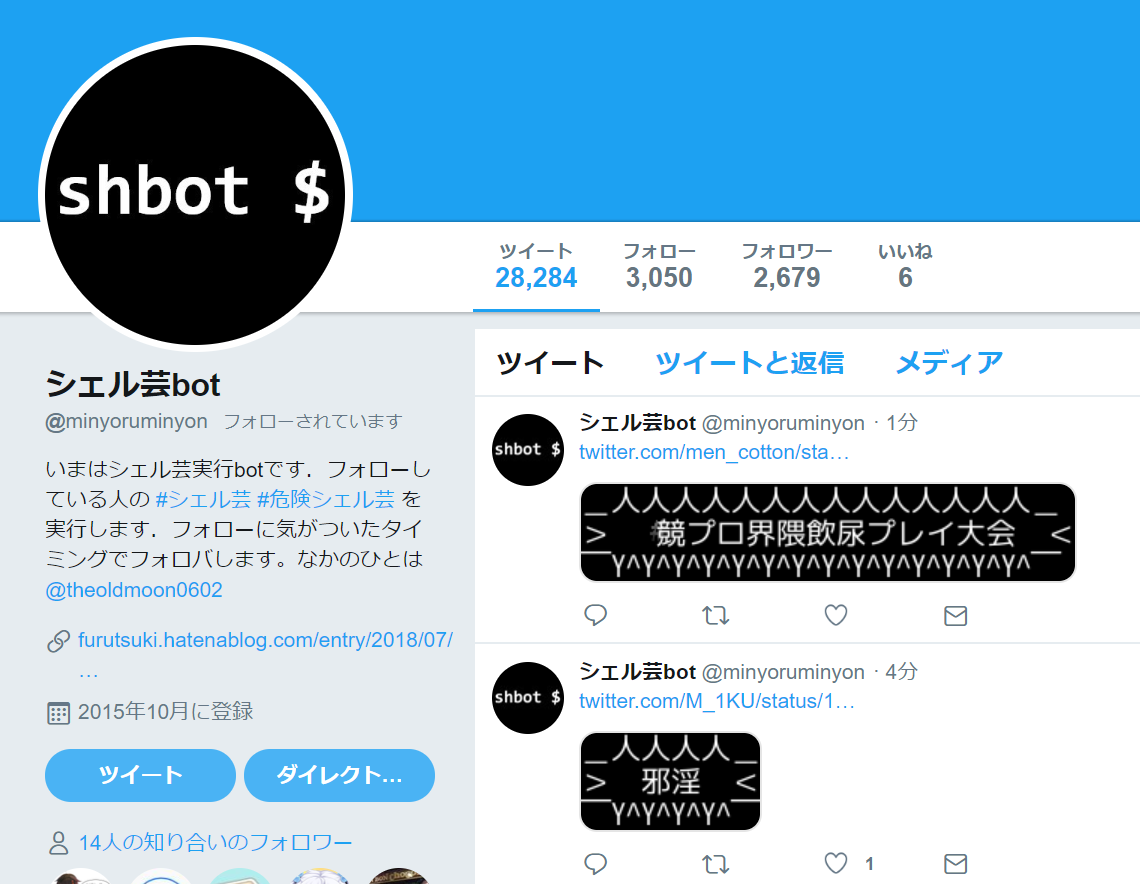
\includegraphics[keepaspectratio, scale=.5]{./img/shellgei.png}\\
  \url{https://twitter.com/minyoruminyon}
\end{frame}

\begin{frame}
  興味のある人は過去のシェル芸勉強会の問題集\footnote{\url{https://b.ueda.tech/?page=00684}}を参照するとよい.
\end{frame}

\begin{frame}{簡単な例}
  サイコロ \\
  \$ seq 6 $|$ shuf $|$ head -1 \\
  \vspace{0.2in}

  連番ディレクトリの作成 \\
  \$ mkdir \$(seq -w 14)
  \vspace{0.2in}
  
  FizzBuzz \\
  \$ seq 31 $|$ sed 5$\sim$5cBuzz $|$ sed 3$\sim$3s/[0-9]*/Fizz/
  \vspace{0.2in}

  OSのユーザー数を求める \\
  \$ cat /etc/passwd $|$ awk -F: '$\{\text{print \$1}\}$' $|$ wc -l
\end{frame}

\section{競プロへの応用}
\begin{frame}
  \centering
  \Huge{競プロへの応用}
\end{frame}

\begin{frame}
  実際にICPCを想定してリダイレクトの演習をします. \\
  けどテストデータ作るのは面倒くさいので, AtCoderの例題でも解いてもらいます. \\
\end{frame}

\begin{frame}
  \fontsize{7pt}{0pt}\selectfont
  77y/5Lq65Lq65Lq65Lq65Lq65Lq65Lq65Lq65Lq65Lq65Lq65Lq65Lq65Lq65Lq65Lq677y/Cu+8 \\
  nuOAgOOBk+OBk+OBi+OCiUBfX0JhY3RwdXNfX+OBruOCv+ODvOODs+OAgO+8nArvv6NZXlleWV5Z \\
  XlleWV5ZXlleWV5ZXlleWV5ZXlleWV5ZXu+/owo=
\end{frame}

\begin{frame}
  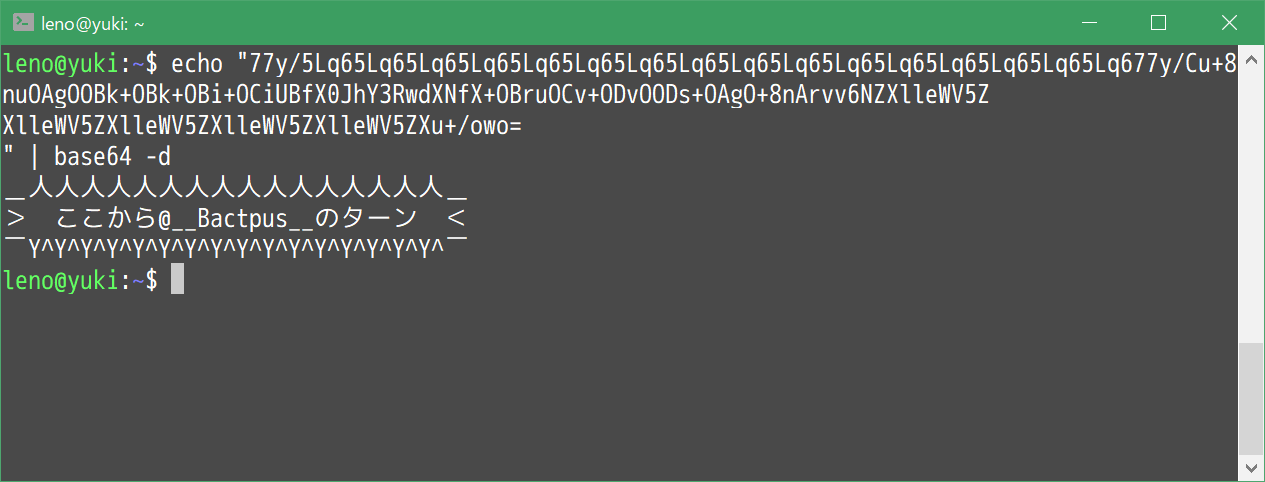
\includegraphics[keepaspectratio, scale=.5]{./img/sd.png}
\end{frame}

\begin{frame}
  \centering
  \Large
  _人人人人人人人人人人人人人人人人_ \\
  > ここから@\_\_Bactpus\_\_のターン < \\
  Y\textasciicircum Y\textasciicircum Y\textasciicircum Y\textasciicircum Y\textasciicircum Y\textasciicircum Y\textasciicircum Y\textasciicircum Y\textasciicircum Y\textasciicircum Y\textasciicircum Y\textasciicircum Y\textasciicircum Y\textasciicircum \\
\end{frame}

\begin{frame}
  \centering
  \Large
  おわり. \\
  \normalsize
  ご清聴ありがとうございました. \\
  ご意見やマサカリ, 質問は\url{twitter.com/leno3s}へ.
\end{frame}

\end{document}


